% Objetivo del archivo: imprimir los planos que se quieran inlcuir como un conjunto.
%
% Sintaxis:
% Incluir un título de conjunto para el índice de planos:
%\conjuntoplanos{Texto del título del conjunto}
%
% Incluir un título de plano:
%\plano{Texto del título del plano}
% Inlcuir un plano como .pdf:
%\begin{figure}
%	\includepdf[scale=X, landscape, pagecommand={}]{RUTA}
%\end{figure}
%
\part{Planos}
%
\conjuntoplanos{Colegio de prácticas del Máster de Incendios}
%
\plano{Planta Baja}
\begin{figure}
	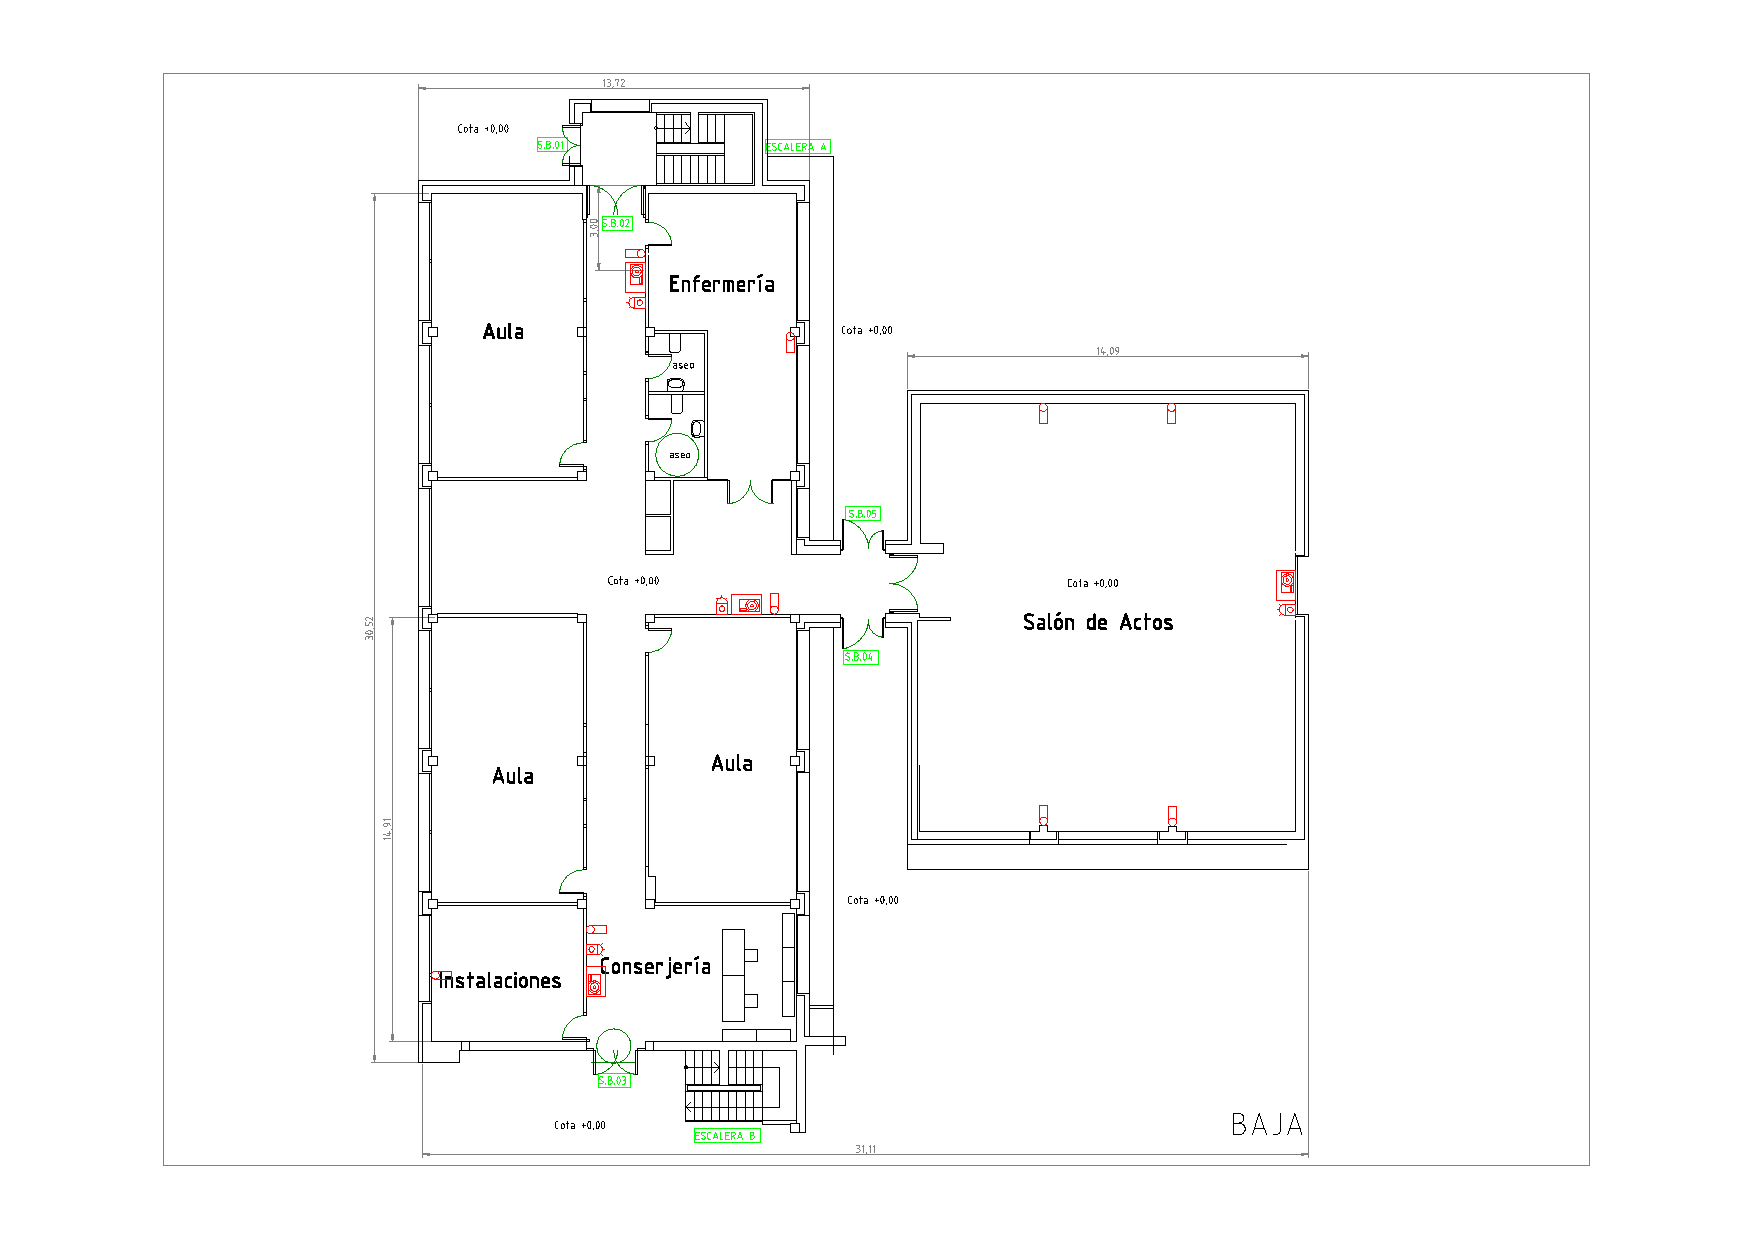
\includepdf[scale=0.95, landscape, pagecommand={}]{planos/plano-planta0.pdf}
\end{figure}
%%
\plano{Planta Primera}
\begin{figure}
	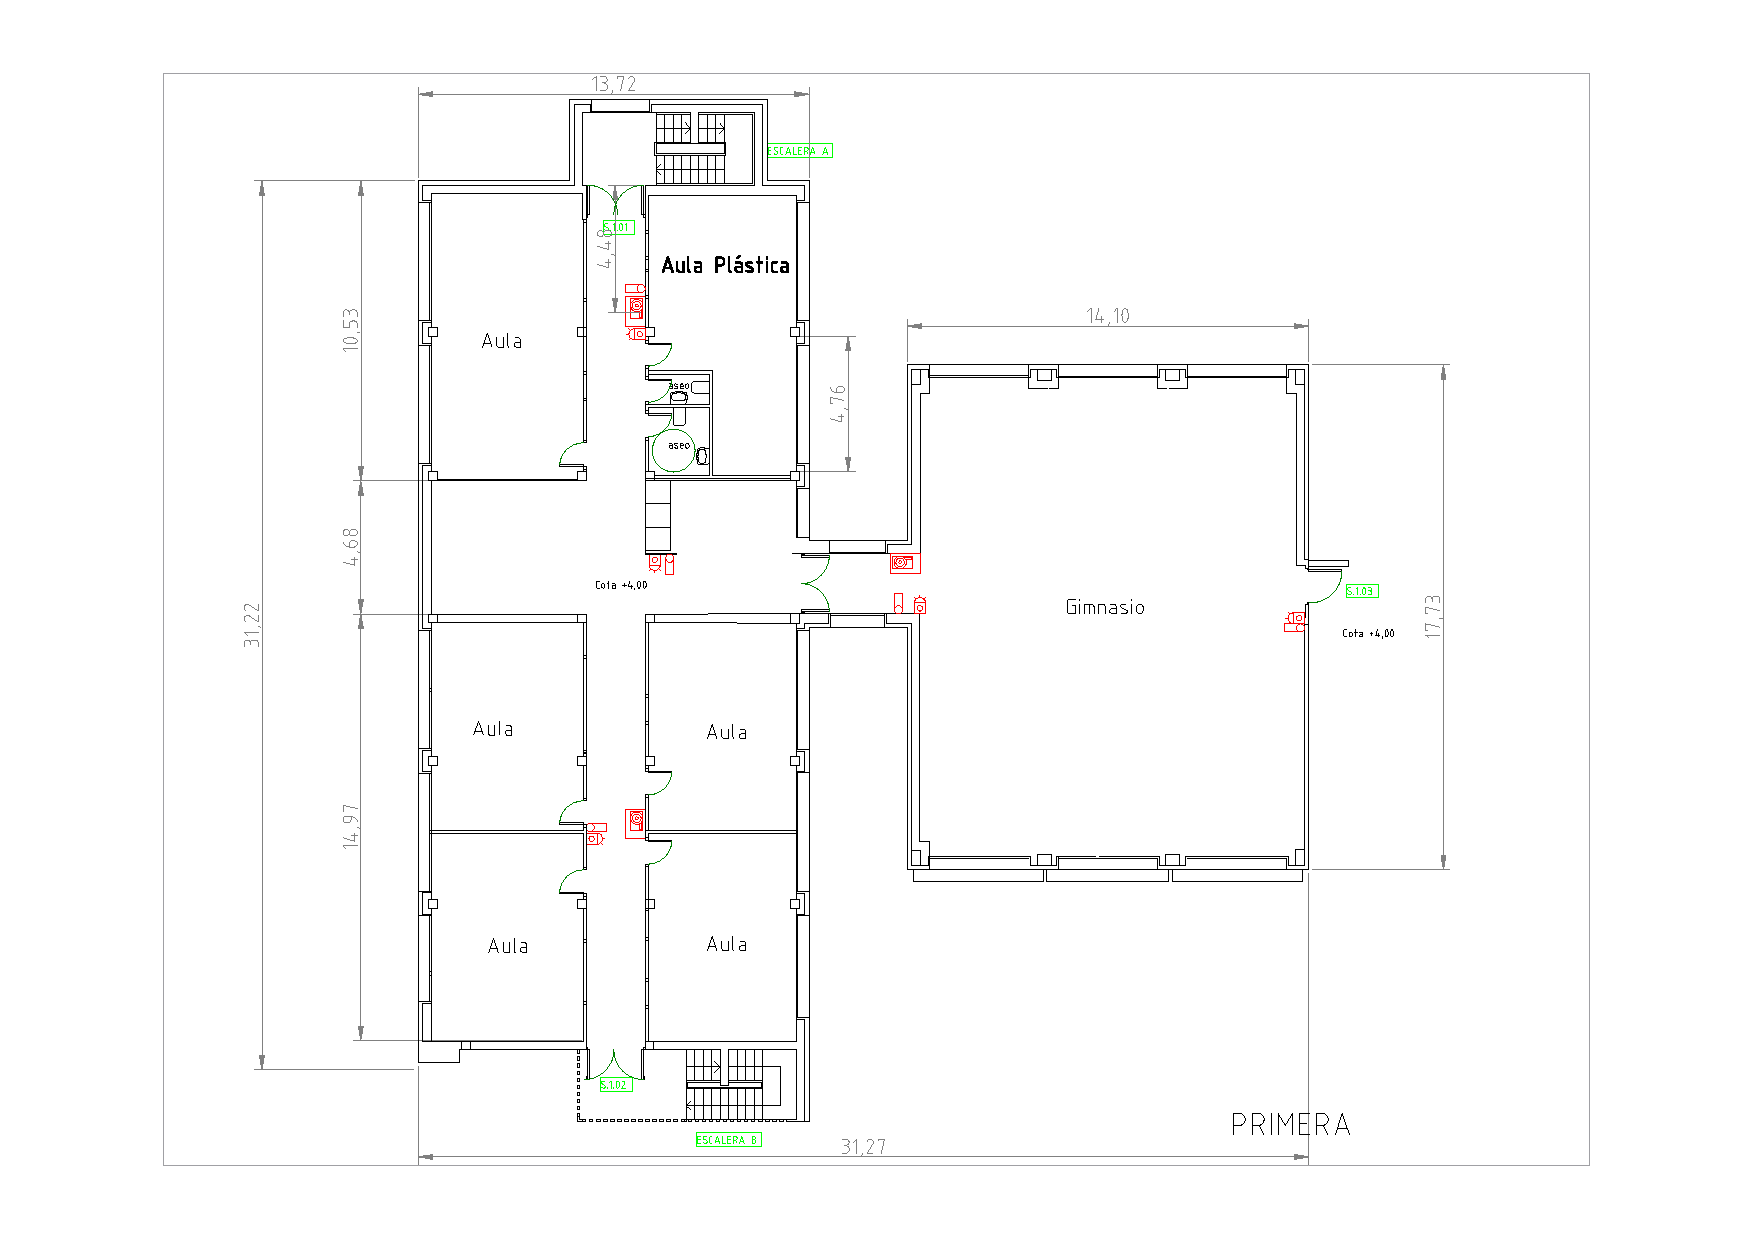
\includepdf[scale=0.95, landscape, pagecommand={}]{planos/plano-planta1.pdf}
\end{figure}
%
\plano{Planta Segunda}
\begin{figure}
	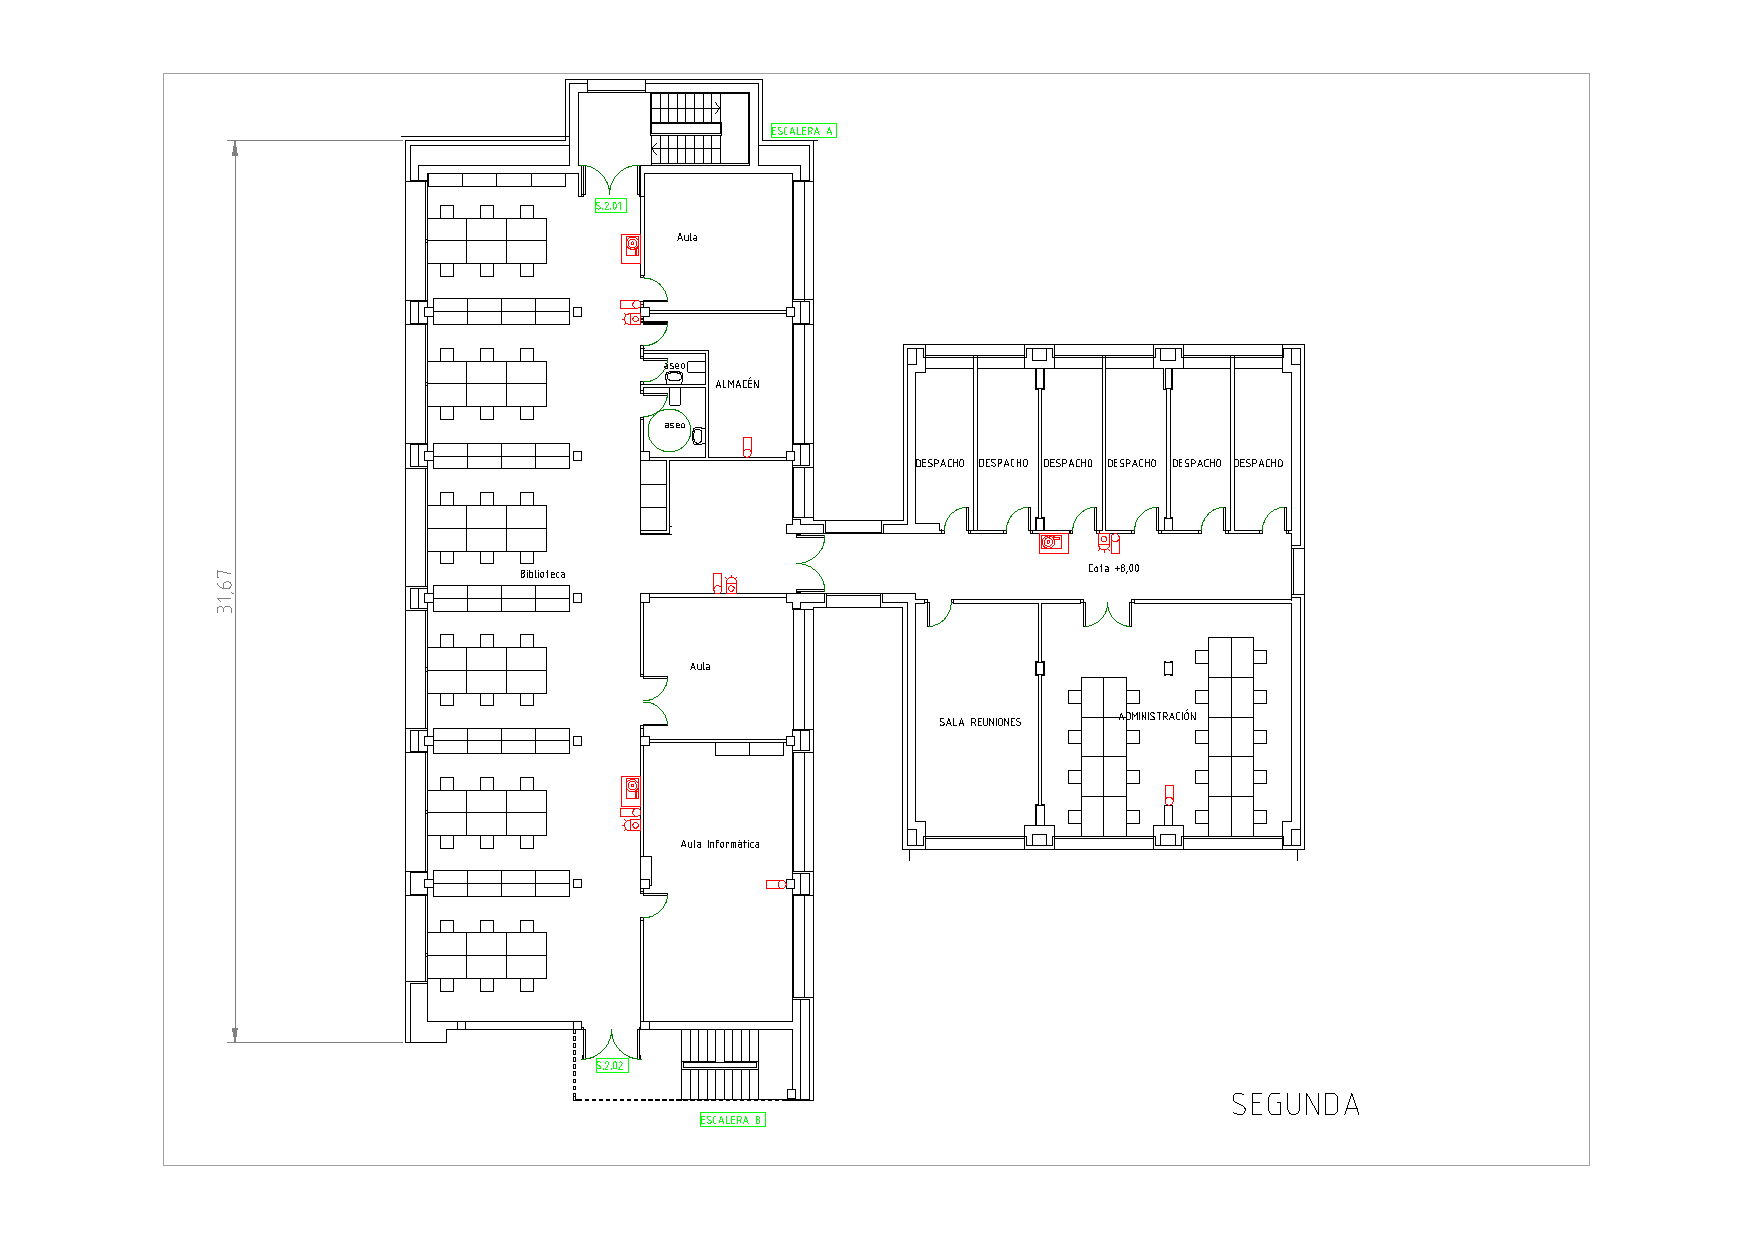
\includepdf[scale=0.95, landscape, pagecommand={}]{planos/plano-planta2.pdf}
\end{figure}
%
\conjuntoplanos{Conjunto de prácticas del Máster de Incendios repetido}
%
\plano{Planta Baja bis}
\begin{figure}
	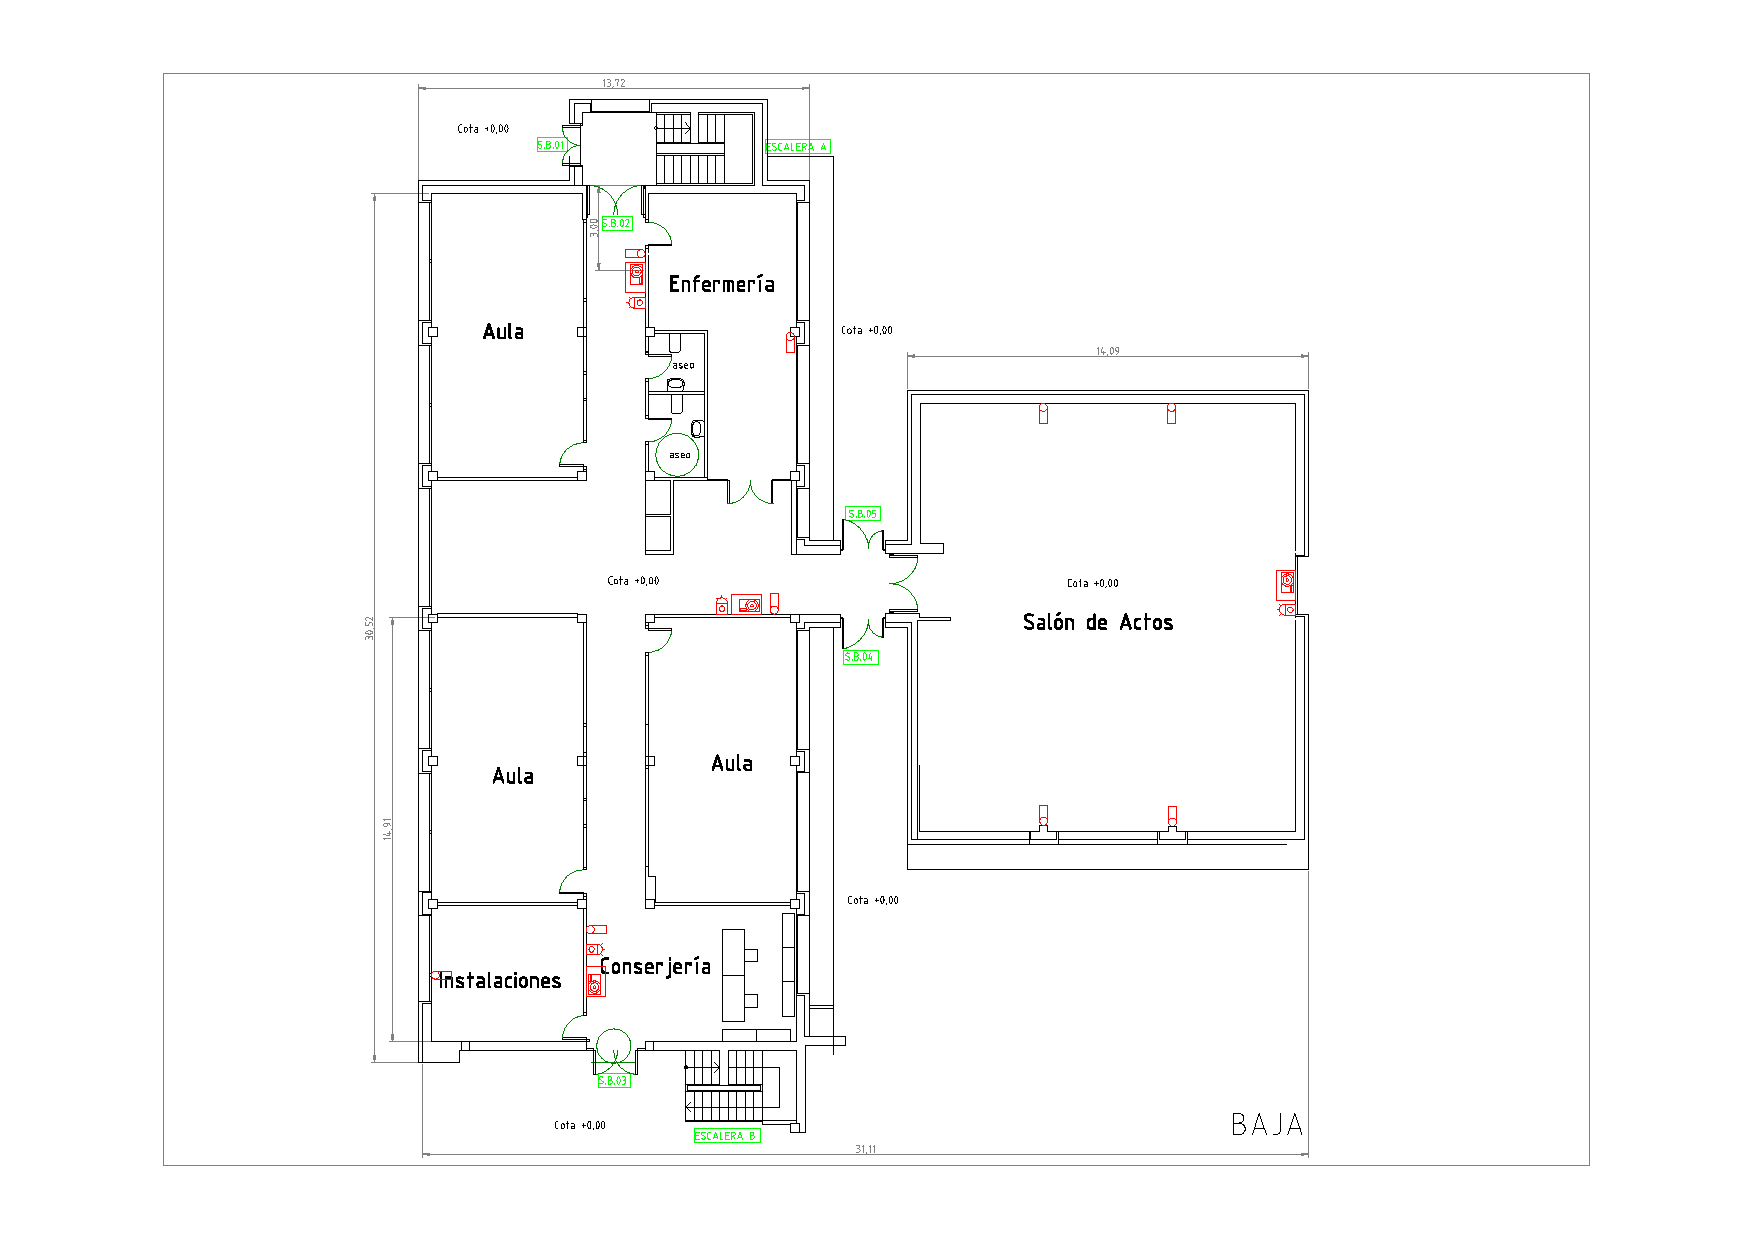
\includepdf[scale=0.95, landscape, pagecommand={}]{planos/plano-planta0.pdf}
\end{figure}
%%
\plano{Planta Primera bis}
\begin{figure}
	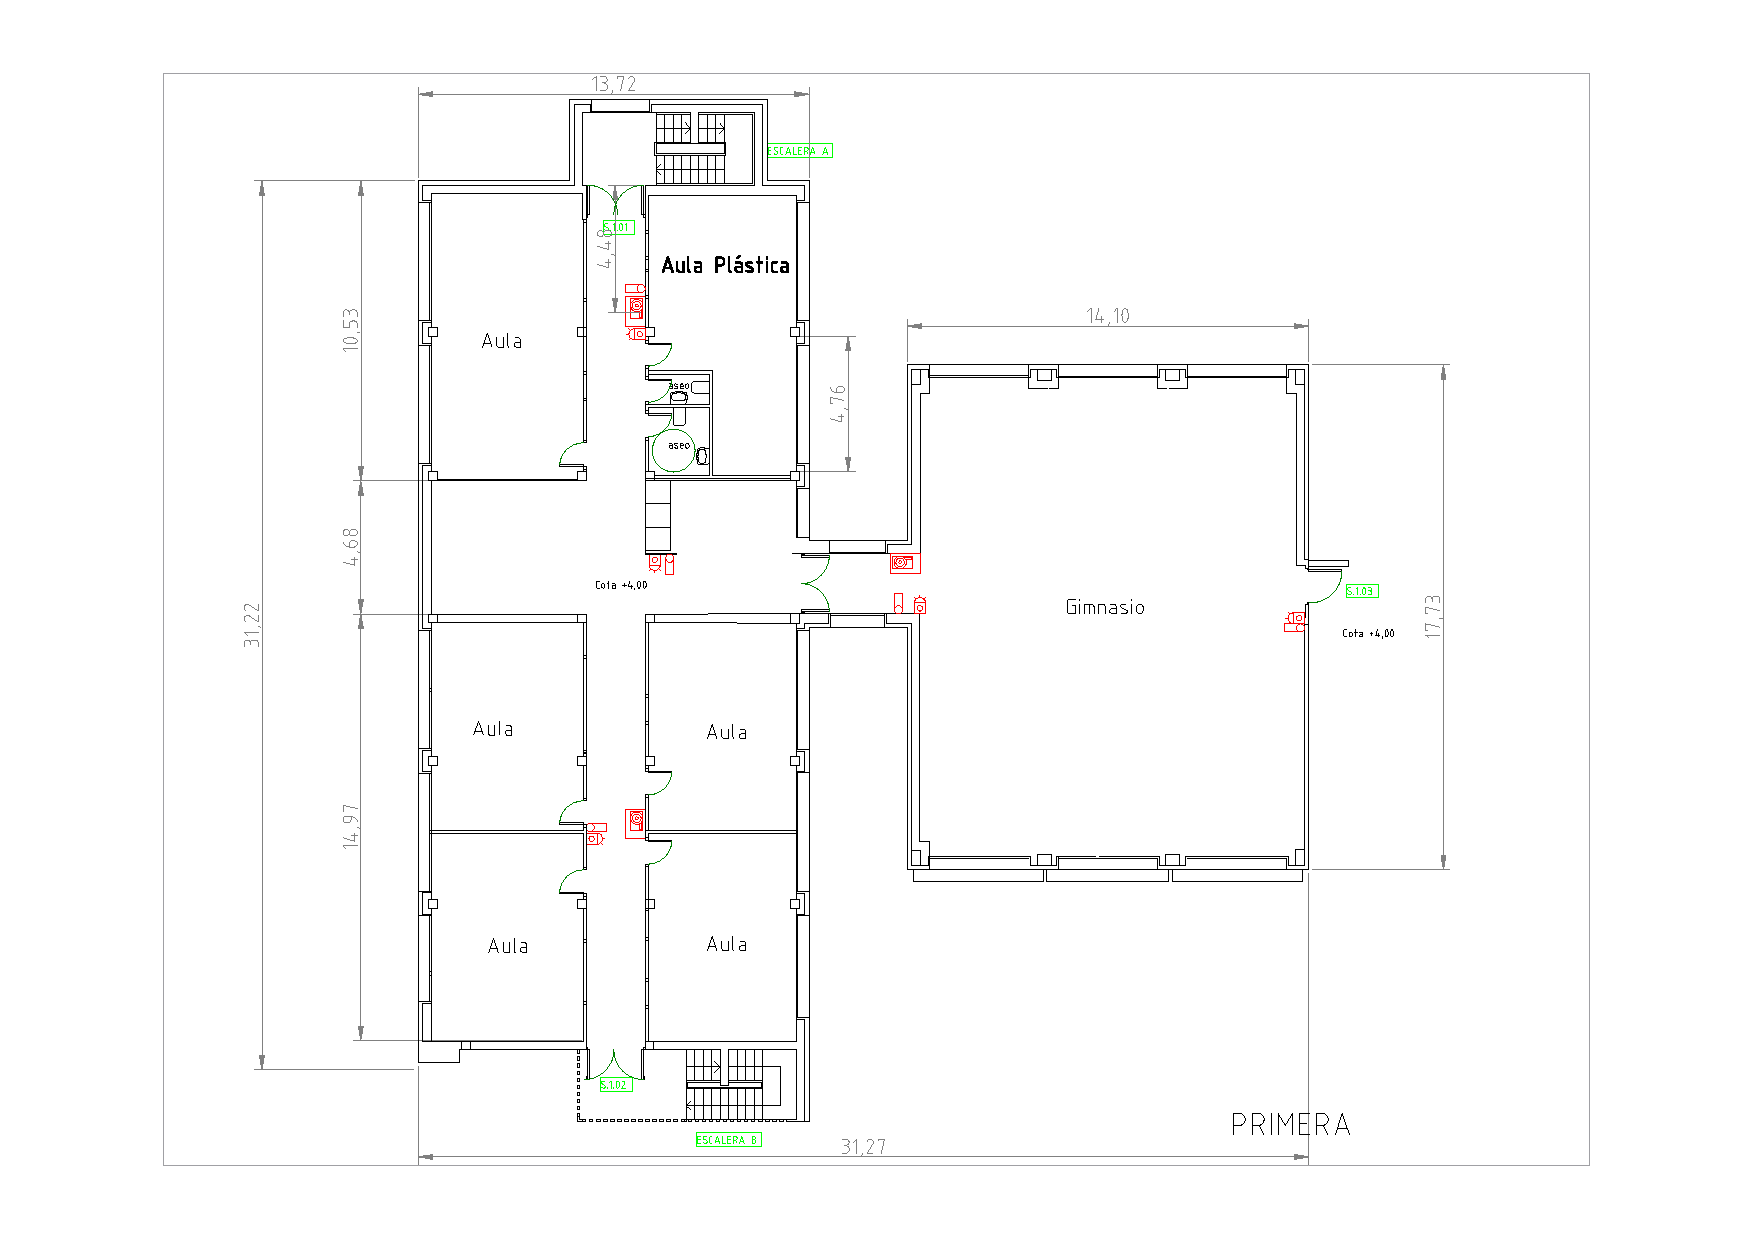
\includepdf[scale=0.95, landscape, pagecommand={}]{planos/plano-planta1.pdf}
\end{figure}
%
\plano{Planta Segunda bis}
\begin{figure}
	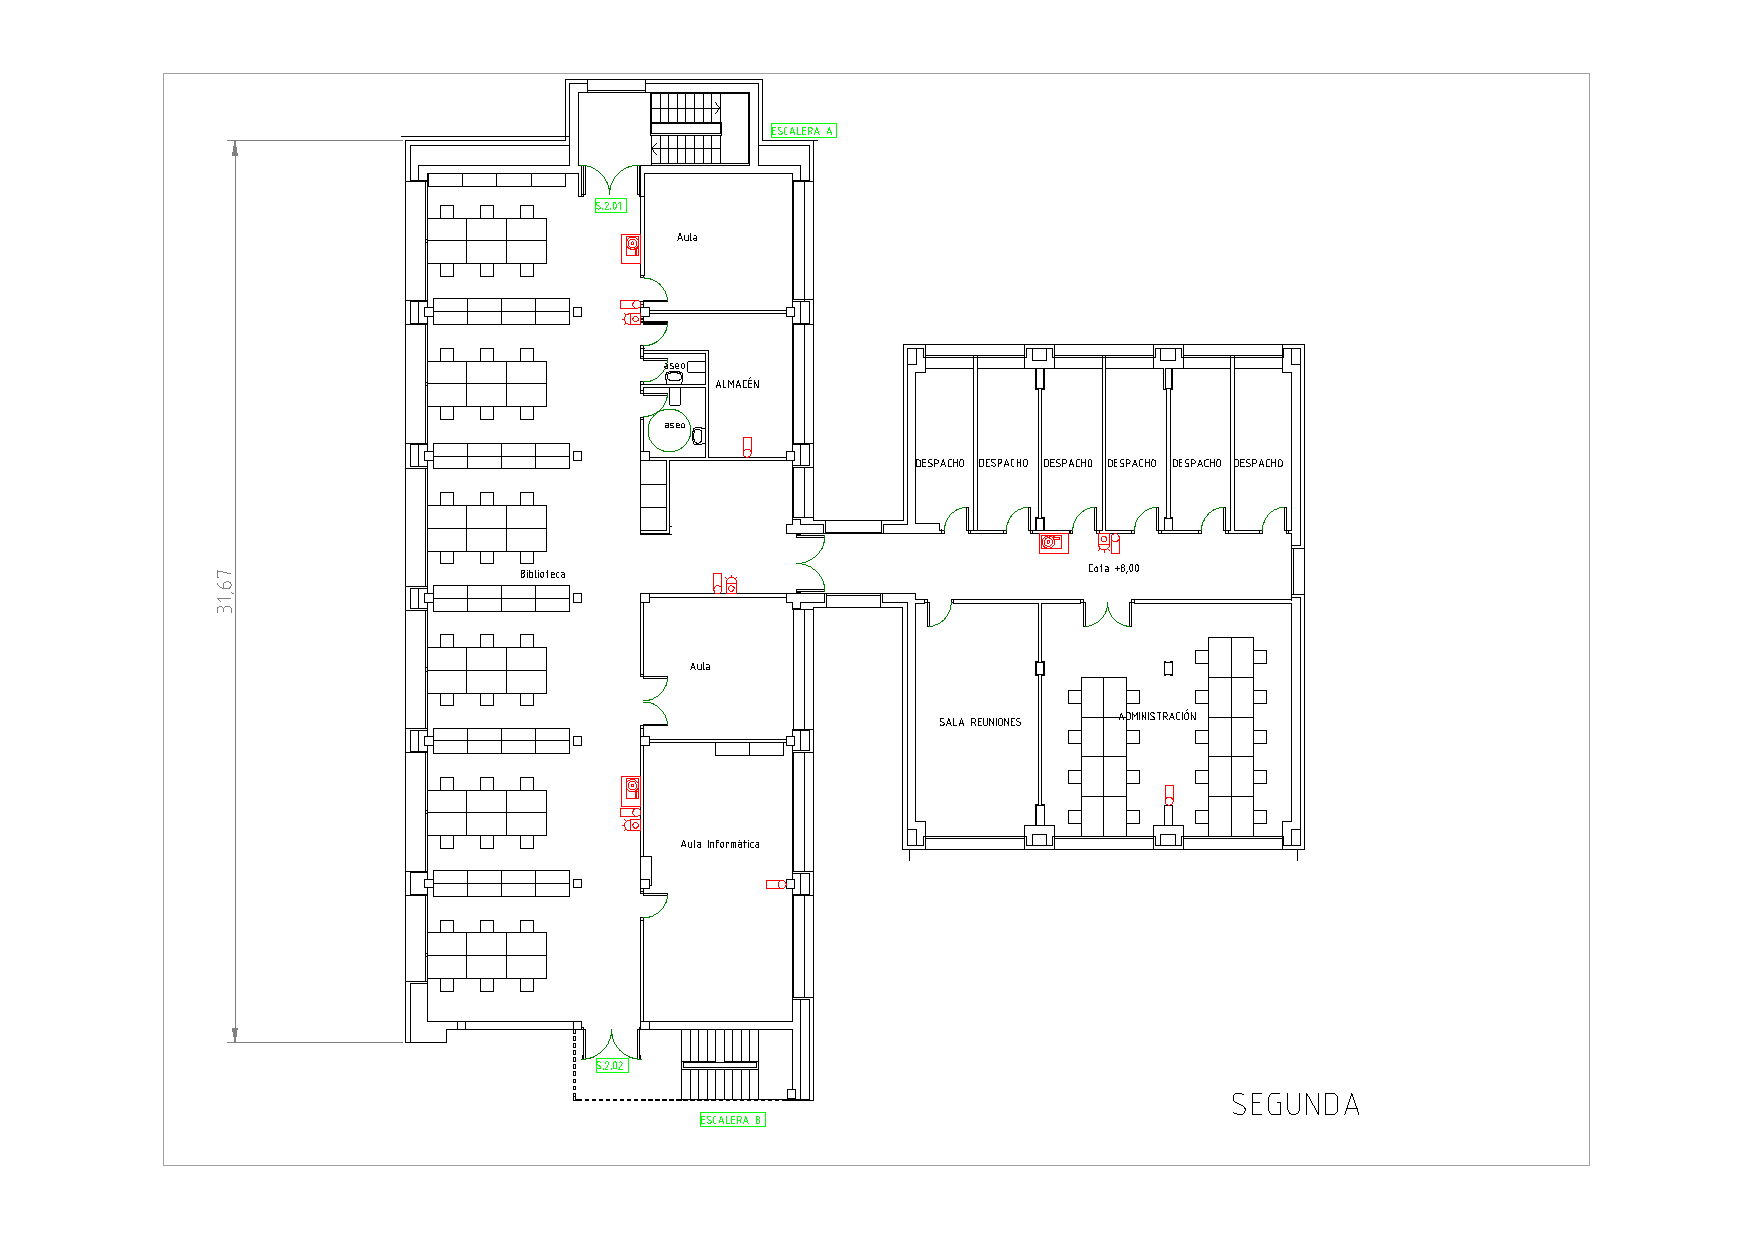
\includepdf[scale=0.95, landscape]{planos/plano-planta2.pdf}
\end{figure}